\documentclass[16pt]{article}
\usepackage[utf8]{inputenc, lscape}
\usepackage[demo]{graphicx}
\usepackage[a4paper,bindingoffset=0.2in,%
            left=1.1in,right=0.85in,top=1in,bottom=1in,%
            footskip=.25in]{geometry}

\begin{document}

% update from cis_prel_results
% 08/25-26. main script is i6_d21_6m__.
% the first two pages are unchanged.
% csd stuff is from i6_d32_csd_

\newgeometry{left=1.5cm, right=1cm, top=3cm, bottom=1.5cm}

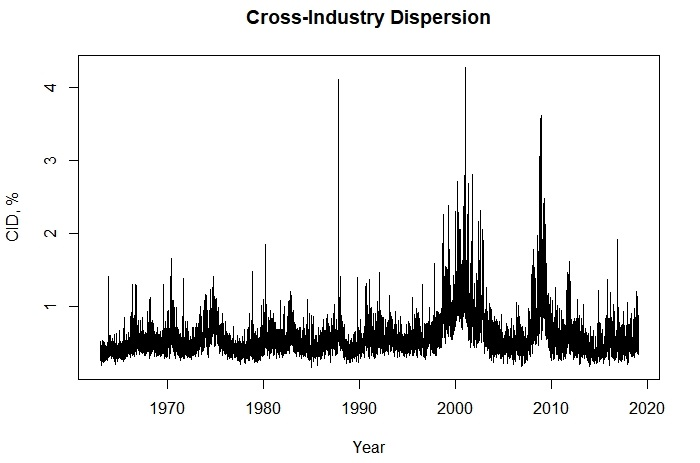
\includegraphics[width=1\textwidth]{ts_cid_00.jpeg}

\newpage

{\textbf{Results in levels:}}

\begin{table}[!htbp] \centering 
  \caption{Excess returns of decile $\beta_{CID}$-sorted portfolios} 
  \label{} 
  
\begin{tabular}{@{\extracolsep{-6pt}} cccccccccccc} 
\\[-1.8ex]\hline 
\hline \\[-1.8ex] 
 & D1 & D2 & D3 & D4 & D5 & D6 & D7 & D8 & D9 & D10 & LS(annualized) \\ 
\hline \\[-1.8ex] 
Mean ew & $0.069$ & $0.052$ & $0.047$ & $0.047$ & $0.044$ & $0.043$ & $0.045$ & $0.042$ & $0.039$ & $0.034$ & $$-$8.828$ \\ 
T\_stat & $7.800$ & $7.044$ & $6.682$ & $6.682$ & $6.221$ & $5.774$ & $5.810$ & $5.133$ & $4.345$ & $3.172$ & $$-$5.021$ \\ 
Mean vw & $0.037$ & $0.027$ & $0.031$ & $0.030$ & $0.026$ & $0.029$ & $0.029$ & $0.022$ & $0.019$ & $0.009$ & $$-$7.215$ \\ 
T\_stat & $3.391$ & $2.949$ & $3.624$ & $3.685$ & $3.253$ & $3.532$ & $3.438$ & $2.428$ & $1.894$ & $0.669$ & $$-$2.733$ \\ 
\hline \\[-1.8ex] 
\end{tabular} 
\end{table}


% Table created by stargazer v.5.2.2 by Marek Hlavac, Harvard University. E-mail: hlavac at fas.harvard.edu
% Date and time: Sun, Aug 18, 2019 - 5:07:25 PM
\begin{table}[!htbp] \centering 
  \caption{Abnormal returns of value-weighted long/short portfolios} 
  \label{} 
\begin{tabular}{@{\extracolsep{5pt}} ccccc} 
\\[-1.8ex]\hline 
\hline \\[-1.8ex] 
Statistic & Ret & Alpha CAPM & Alpha FF3 & Alpha FF5 \\ 
\hline \\[-1.8ex] 
Return & -7.308 & -8.316 & -11.088 & -10.332 \\ 
T-stat & [ -2.730] & [ -3.216] & [ -4.516] & [ -4.165] \\ 
\hline \\[-1.8ex] 
\end{tabular} 
\end{table}



% Table created by stargazer v.5.2.2 by Marek Hlavac, Harvard University. E-mail: hlavac at fas.harvard.edu
% Date and time: Sun, Aug 18, 2019 - 5:11:11 PM
\begin{table}[!htbp] \centering 
  \caption{Factor loadings} 
  \label{} 
\begin{tabular}{@{\extracolsep{-3pt}} ccccccccc} 
\\[-1.8ex]\hline 
\hline \\[-1.8ex] 
Ntile & Ret & Alpha & EMKT & HML & SMB & RMW & CMA & adjR2 \\ 
\hline \\[-1.8ex] 
1 & 0.037 & 0.016 & 1.063 & -0.192 & 0.407 & -0.219 & -0.174 & 0.757 \\ 
 & [ 3.371] & [ 2.994] & [ 172.759] & [ -14.774] & [ 36.783] & [ -13.702] & [ -9.235] &  \\ 
2 & 0.027 & 0.004 & 0.969 & -0.093 & 0.249 & -0.010 & -0.038 & 0.800 \\ 
 & [ 2.929] & [ 0.884] & [ 207.352] & [ -9.440] & [ 29.632] & [ -0.852] & [ -2.660] &  \\ 
3 & 0.031 & 0.008 & 0.927 & -0.084 & 0.155 & 0.014 & 0.038 & 0.829 \\ 
 & [ 3.598] & [ 2.165] & [ 231.465] & [ -9.884] & [ 21.514] & [ 1.352] & [ 3.066] &  \\ 
4 & 0.030 & 0.005 & 0.928 & -0.060 & 0.105 & 0.077 & 0.119 & 0.855 \\ 
 & [ 3.662] & [ 1.666] & [ 260.242] & [ -7.961] & [ 16.358] & [ 8.291] & [ 10.888] &  \\ 
5 & 0.026 & -0.001 & 0.932 & 0.005 & 0.083 & 0.129 & 0.126 & 0.874 \\ 
 & [ 3.229] & [ -0.189] & [ 285.878] & [ 0.681] & [ 14.143] & [ 15.209] & [ 12.638] &  \\ 
6 & 0.029 & 0.001 & 0.952 & 0.045 & 0.048 & 0.140 & 0.127 & 0.890 \\ 
 & [ 3.514] & [ 0.387] & [ 308.445] & [ 6.953] & [ 8.634] & [ 17.426] & [ 13.438] &  \\ 
7 & 0.029 & 0.000 & 0.983 & 0.106 & 0.019 & 0.147 & 0.094 & 0.891 \\ 
 & [ 3.419] & [ 0.030] & [ 309.228] & [ 15.803] & [ 3.252] & [ 17.753] & [ 9.717] &  \\ 
8 & 0.022 & -0.008 & 1.041 & 0.197 & 0.003 & 0.107 & 0.037 & 0.883 \\ 
 & [ 2.406] & [ -2.743] & [ 296.741] & [ 26.509] & [ 0.499] & [ 11.716] & [ 3.483] &  \\ 
9 & 0.019 & -0.015 & 1.125 & 0.402 & 0.037 & 0.111 & -0.145 & 0.855 \\ 
 & [ 1.879] & [ -3.788] & [ 258.997] & [ 43.741] & [ 4.757] & [ 9.814] & [ -10.928] &  \\ 
10 & 0.008 & -0.025 & 1.284 & 0.700 & 0.130 & -0.172 & -0.591 & 0.776 \\ 
 & [ 0.655] & [ -4.068] & [ 187.207] & [ 48.206] & [ 10.565] & [ -9.634] & [ -28.204] &  \\ 
LS & -0.029 & -0.041 & 0.221 & 0.892 & -0.277 & 0.047 & -0.418 & 0.130 \\ 
 & [ -2.730] & [ -4.165] & [ 19.834] & [ 37.894] & [ -13.838] & [ 1.642] & [ -12.279] &  \\ 
\hline \\[-1.8ex] 
\end{tabular} 
\end{table}



\begin{table}[!htbp] \centering 
  \caption{Fama-MacBeth egression of excess returns on characteristics} 
  \label{} 
\begin{tabular}{@{\extracolsep{5pt}} ccccc} 
\\[-1.8ex]\hline 
\hline \\[-1.8ex] 
 & Intercept & beta\_cimad & beta & size \\ 
\hline \\[-1.8ex] 
coefmean & $0.2278$ & $$-$0.0069$ & $0.0095$ & $$-$0.0165$ \\ 
se & $0.0132$ & $0.0013$ & $0.0080$ & $0.0011$ \\ 
tstat & $17.2100$ & $$-$5.1390$ & $1.1860$ & $$-$15.7000$ \\ 
r2 & $0.0215$ & $0.0215$ & $0.0215$ & $0.0215$ \\ 
\hline \\[-1.8ex] 
\end{tabular} 
\end{table}


\newpage

{\textbf{Results in differences:}}

% Table created by stargazer v.5.2.2 by Marek Hlavac, Harvard University. E-mail: hlavac at fas.harvard.edu
% Date and time: Sun, Aug 25, 2019 - 5:45:14 PM
\begin{table}[!htbp] \centering 
  \caption{Returns of $\beta_{CID}-sorted portfolios$} 
  \label{} 
\begin{tabular}{@{\extracolsep{5pt}} cccccccccccc} 
\\[-1.8ex]\hline 
\hline \\[-1.8ex] 
 & D1 & D2 & D3 & D4 & D5 & D6 & D7 & D8 & D9 & D10 & LS \\ 
\hline \\[-1.8ex] 
Mean ew & $18.50$ & $14.60$ & $13.05$ & $12.85$ & $12.69$ & $12.33$ & $12.08$ & $12.17$ & $12.10$ & $12.83$ & $$-$5.45$ \\ 
T-stat & $8.26$ & $7.70$ & $7.29$ & $7.32$ & $7.18$ & $6.86$ & $6.47$ & $6.16$ & $5.61$ & $4.81$ & $$-$3.18$ \\ 
Mean vw& $12.10$ & $8.32$ & $7.59$ & $7.78$ & $7.83$ & $7.22$ & $6.62$ & $6.22$ & $5.08$ & $4.17$ & $$-$7.81$ \\ 
T-stat & $4.67$ & $3.78$ & $3.67$ & $3.83$ & $3.87$ & $3.56$ & $3.16$ & $2.84$ & $2.11$ & $1.40$ & $$-$3.28$ \\ 
\hline \\[-1.8ex] 
\end{tabular} 
\end{table}


% Table created by stargazer v.5.2.2 by Marek Hlavac, Harvard University. E-mail: hlavac at fas.harvard.edu
% Date and time: Sun, Aug 25, 2019 - 5:47:32 PM
\begin{table}[!htbp] \centering 
  \caption{Abnormal returns of vw portfolios} 
  \label{} 
\begin{tabular}{@{\extracolsep{5pt}} cccccc} 
\\[-1.8ex]\hline 
\hline \\[-1.8ex] 
Ntile & Ret & Alpha CAPM & Alpha FF3 & Alpha FF5 & Alpha FF5+UMD+Liq \\ 
\hline \\[-1.8ex] 
LS & -7.812 & -9.072 & -11.088 & -9.576 & -5.544 \\ 
 & [ -3.284] & [ -3.849] & [ -4.824] & [ -4.224] & [ -2.457] \\ 
\hline \\[-1.8ex] 
\end{tabular} 
\end{table}



% Table created by stargazer v.5.2.2 by Marek Hlavac, Harvard University. E-mail: hlavac at fas.harvard.edu
% Date and time: Sun, Aug 25, 2019 - 5:51:00 PM
\begin{table}[!htbp] \centering 
  \caption{Factor loadings} 
  \label{} 
\begin{tabular}{@{\extracolsep{5pt}} ccccccccc} 
\\[-1.8ex]\hline 
\hline \\[-1.8ex] 
Ntile & Ret & Alpha & EMKT & HML & SMB & RMW & CMA & adjR2 \\ 
\hline \\[-1.8ex] 
1 & 12.096 & 6.3 & 1.038 & -0.199 & 0.320 & -0.082 & -0.117 & 0.759 \\ 
 & [ 4.661] & [ 4.878] & [ 178.469] & [ -16.344] & [ 30.778] & [ -5.494] & [ -6.667] &  \\ 
2 & 8.316 & 1.764 & 0.959 & -0.094 & 0.195 & 0.099 & 0.082 & 0.809 \\ 
 & [ 3.757] & [ 1.818] & [ 220.041] & [ -10.250] & [ 24.893] & [ 8.706] & [ 6.159] &  \\ 
3 & 7.56 & 1.26 & 0.924 & -0.065 & 0.133 & 0.100 & 0.109 & 0.840 \\ 
 & [ 3.655] & [ 1.401] & [ 246.764] & [ -8.186] & [ 19.668] & [ 10.252] & [ 9.512] &  \\ 
4 & 7.812 & 1.512 & 0.919 & -0.040 & 0.075 & 0.089 & 0.101 & 0.863 \\ 
 & [ 3.811] & [ 1.923] & [ 269.543] & [ -5.481] & [ 12.164] & [ 10.010] & [ 9.736] &  \\ 
5 & 7.812 & 1.26 & 0.929 & -0.003 & 0.044 & 0.129 & 0.126 & 0.873 \\ 
 & [ 3.850] & [ 1.568] & [ 284.017] & [ -0.394] & [ 7.483] & [ 15.144] & [ 12.656] &  \\ 
6 & 7.056 & 0.252 & 0.943 & 0.025 & 0.004 & 0.126 & 0.166 & 0.885 \\ 
 & [ 3.535] & [ 0.394] & [ 302.676] & [ 3.791] & [ 0.707] & [ 15.581] & [ 17.491] &  \\ 
7 & 6.552 & -0.504 & 0.966 & 0.077 & -0.013 & 0.134 & 0.089 & 0.882 \\ 
 & [ 3.140] & [ -0.549] & [ 296.225] & [ 11.160] & [ -2.198] & [ 15.773] & [ 8.896] &  \\ 
8 & 6.048 & -1.008 & 1.005 & 0.121 & -0.040 & 0.139 & 0.040 & 0.883 \\ 
 & [ 2.814] & [ -1.372] & [ 296.404] & [ 16.883] & [ -6.630] & [ 15.798] & [ 3.831] &  \\ 
9 & 5.04 & -2.268 & 1.073 & 0.227 & -0.023 & 0.047 & -0.100 & 0.860 \\ 
 & [ 2.090] & [ -2.512] & [ 262.884] & [ 26.333] & [ -3.135] & [ 4.425] & [ -8.037] &  \\ 
10 & 4.032 & -3.024 & 1.208 & 0.427 & 0.030 & -0.175 & -0.469 & 0.778 \\ 
 & [ 1.382] & [ -2.083] & [ 189.524] & [ 31.650] & [ 2.634] & [ -10.563] & [ -24.086] &  \\ 
LS & -7.812 & -9.576 & 0.189 & 0.638 & -0.276 & -0.105 & -0.342 & 0.099 \\ 
 & [ -3.284] & [ -4.224] & [ 18.228] & [ 29.379] & [ -14.920] & [ -3.944] & [ -10.925] &  \\ 
\hline \\[-1.8ex] 
\end{tabular} 
\end{table}



% Table created by stargazer v.5.2.2 by Marek Hlavac, Harvard University. E-mail: hlavac at fas.harvard.edu
% Date and time: Sun, Aug 25, 2019 - 6:09:17 PM
\begin{table}[!htbp] \centering 
  \caption{Characteristics of vw decile portfolios} 
  \label{} 
\begin{tabular}{@{\extracolsep{5pt}} cccccccccccc} 
\\[-1.8ex]\hline 
\hline \\[-1.8ex] 
 & D1 & D2 & D3 & D4 & D5 & D6 & D7 & D8 & D9 & D10 & LS \\ 
\hline \\[-1.8ex] 
RET & $12.10$ & $8.32$ & $7.59$ & $7.78$ & $7.83$ & $7.22$ & $6.62$ & $6.22$ & $5.08$ & $4.17$ & $$-$7.81$ \\ 
RET\_tstat & $4.67$ & $3.78$ & $3.67$ & $3.83$ & $3.87$ & $3.56$ & $3.16$ & $2.84$ & $2.11$ & $1.40$ & $$-$3.28$ \\ 
size & $14.47$ & $15.04$ & $15.31$ & $15.52$ & $15.65$ & $15.78$ & $15.86$ & $15.91$ & $15.82$ & $15.43$ & $0.95$ \\ 
bm & $$-$1.01$ & $$-$0.91$ & $$-$0.89$ & $$-$0.88$ & $$-$0.87$ & $$-$0.87$ & $$-$0.89$ & $$-$0.94$ & $$-$0.95$ & $$-$1.00$ & $0.01$ \\ 
op & $0.16$ & $0.17$ & $0.17$ & $0.17$ & $0.17$ & $0.17$ & $0.17$ & $0.18$ & $0.18$ & $0.17$ & $0.01$ \\ 
inv & $0.25$ & $0.18$ & $0.15$ & $0.14$ & $0.14$ & $0.13$ & $0.14$ & $0.14$ & $0.15$ & $0.20$ & $$-$0.05$ \\ 
beta & $1.01$ & $0.92$ & $0.90$ & $0.89$ & $0.90$ & $0.92$ & $0.95$ & $1.00$ & $1.08$ & $1.24$ & $0.23$ \\ 
BAspr & $0.33$ & $0.25$ & $0.22$ & $0.21$ & $0.20$ & $0.19$ & $0.19$ & $0.19$ & $0.19$ & $0.22$ & $$-$0.12$ \\ 
mom122 & $21.20$ & $15.52$ & $13.55$ & $12.90$ & $12.14$ & $11.73$ & $11.60$ & $11.56$ & $12.06$ & $13.94$ & $$-$7.26$ \\ 
vol1m & $2.25$ & $1.81$ & $1.67$ & $1.59$ & $1.57$ & $1.56$ & $1.59$ & $1.64$ & $1.77$ & $2.17$ & $$-$0.08$ \\ 
vol12m & $2.24$ & $1.85$ & $1.72$ & $1.66$ & $1.64$ & $1.63$ & $1.66$ & $1.71$ & $1.84$ & $2.22$ & $$-$0.02$ \\ 
\hline \\[-1.8ex] 
\end{tabular} 
\end{table}



% Table created by stargazer v.5.2.2 by Marek Hlavac, Harvard University. E-mail: hlavac at fas.harvard.edu
% Date and time: Mon, Aug 26, 2019 - 9:29:26 AM
\begin{table}[!htbp] \centering 
  \caption{Abnormal returns of L/S portfolios from 5x5 doublesorts on CSD and CID} 
  \label{} 
\begin{tabular}{@{\extracolsep{5pt}} ccccc} 
\\[-1.8ex]\hline 
\hline \\[-1.8ex] 
Portfolio & Ret & Alpha CAPM & Alpha FF3 & Alpha FF5 \\ 
\hline \\[-1.8ex] 
LS CSD, RET & 1.764 & 2.52 & 2.52 & -0.252 \\ 
LS CSD, T-stat & [ 1.110] & [ 1.505] & [ 1.443] & [ -0.113] \\ 
LS CID, RET & 4.284 & 4.788 & 5.292 & 6.048 \\ 
LS CSD, T-stat & [ 2.682] & [ 2.827] & [ 3.417] & [ 3.873] \\ 
\hline \\[-1.8ex] 
\end{tabular} 
\end{table}



\end{document}
